\documentclass{article}

\usepackage[utf8]{inputenc}
\usepackage[francais]{babel}
\usepackage{amsmath}
\usepackage{amssymb}
\usepackage{fancyhdr}
\pagestyle{fancy}


\lhead{Coralie Saysset - Romain Gerard}
\chead{}
\rhead{B3301}

\usepackage{graphicx}
\begin{document}

\begin{center} 
\Huge{Références croisées sur un ensemble de fichier C++}
\end{center}

\section{Spécifications}
Le but du programme est de permettre de retrouver les emplacements d'identifcateurs dans une collection de fichiers. L'emplacement de chaque occurence sera désigné
par le nom du fichier ainsi que le numero de ligne où elle a été rencontrée. On ne considèrera pas la position sur la ligne.

Dans le cas où un identifacteur apparaitrait plusieurs fois sur une même ligne, nous avons pris la décision d'afficher la ligne conserné une fois par occurence. Etant donné qu'un même identificateur ne devrait pas être présent de trop nombreuses fois sur une même ligne, nous avons jugé que cette présentation ne nuirait pas à la lisibilité de notre programme.


\subsection{Définition du vocabulaire}

\begin{itemize}
\item \textbf{ligne} : On considèrera une ligne comme une suite de caractère terminé par un retour chariot

\item \textbf{Identificateur} : C'est un mot sensible à la casse composé uniquement de caractères alphanumériques et du caractère `\_`. Les identificateurs présents dans des commentaires ou des chaines littérales ne seront pas pris en compte. 

\item \textbf{Déliminateur} : C'est un unique caractère qui représente une séparation entre deux mots 

\item \textbf{Référence croisée} : Une référence croisée est une occurence d'un identificateur

\end{itemize}


\subsection{Spécifications des options}

\begin{center}
\textbf{$tp\_stl\ [-e]\ [-k fichier\_mot\_clef]\ [nomfichier]+$}
\end{center}

\begin{itemize}

 \item[] \textbf{-e} : Permet d'inverser le comportement par défaut du programme. Elle exclue de la référence croisée tous les mots clefs
 
 \item[] \textbf{-k fichier\_mot\_clef} : Permet de spécifier au programme une liste de mot clef à rechercher pour la référence croisée

 \item[] \textbf{nomfichier} : Chemin d'un fichier où chercher les références des identifacateurs

\end{itemize}

\subsection{Identification des classes}

\subsubsection{Structure pour stocker les mots clefs}

\paragraph{Besoins utilisateurs :}
Les mots clefs sont stockés dans un fichier. Pour en faciliter l'accès dans le programme nous souhaitons les charger en mémoire. Ce pose alors la question du choix de la structure de donnée pour les contenir ?

Nous avons besoins d'une structure permettant de nous dire facilement si un mot clef est présent ou non dans la structure de données. Un mot clef ne peut être présent qu'une seule fois dans la structure, car les doublons n'ont pas de sens dans ce problème. De plus l'ordre n'a que peu d'importance.

Nous avons donc besoin uniquement de connaitre rapidement la présence ou non d'un mot clef.

\paragraph{Analyse d'une liste :} 

Comme nous l'avons vu dans nos besoins, seul l'accès en lecture nous intérèsse. Une liste est une structure plate, c'est à dire qu'il n'y a qu'une direction possible.
Dans le pire des cas il nous faut donc parcourir tous les éléments de la liste pour savoir si le mot clef est présent.
La complexité d'une telle structure pour la recherche est donc linéaire ( O(n) ).

\begin{figure}[htp]
\centering
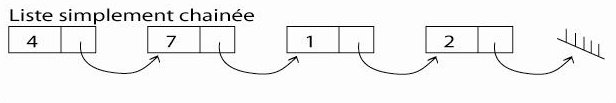
\includegraphics[scale=0.6]{images/liste.jpg}
\caption{Liste chainée}
\label{}
\end{figure}

\paragraph{Analyse d'un arbre :}
Un arbre est une structure possédant plusieurs directions. De plus si l'on utilise un arbre binaire
le choix de la direction est déterminé par le noeud courant et la valeur que l'on cherche. 

Dans le pire des cas, si l'arbre n'est pas isométrique il
faut parcourir tous les noeuds pour savoir si la clef est présente ou non. Par contre dans les cas moyen avec un arbre équilibré la recherche se fait en log(n).

\paragraph{Choix de la structure :}
Une structure en arbre nous semble plus adapté car nous souhaitons favoriser la recherche. Dans les cas moyens la liste reste en compléxité linéaire tandis qu'un arbre est de compléxité logarithmique.

Nous avons donc décidé de stocker la liste des mots clefs dans une stucture sous forme d'arbre.

 
\begin{figure}[htp]
\centering
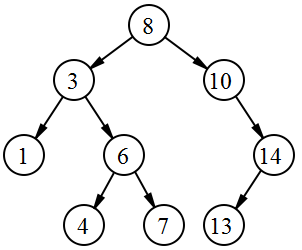
\includegraphics[scale=0.5]{images/arbre.png}
\caption{Arbre binaire}
\label{}
\end{figure}

\subsection{Structure pour stocker les identifiants}

\paragraph{Besoins :}
Chaque identificateur présents dans la collection de fichier(s) doit être stocké en mémoire avec la liste de ses occurences. Un identificateur a donc une clef (lui même) et une valeur (sa liste d'occurence). Nous souhaitons optimiser l'insertion et la lecture des valeurs des identificateurs. On se pose alors la question du choix de la stucture de donnée a adopter.


\paragraph{Analyse d'un arbre rouge et noir :}


\paragraph{Analyse d'une table de hash :}

\paragraph{}
 
\subsection{Plan des tests fonctionnels}





\end{document}